\section{Gamma Spectra}

\begin{frame}{Gamma Spectra}
    	\vspace{-0.05\textheight}
   	\begin{columns}
		\begin{column}{0.6\textwidth}
			\begin{overlayarea}{\textwidth}{\textheight}
				\centering
				\only<1>{\includegraphics[width=\textwidth]{GammaNotGated}}
				\only<2>{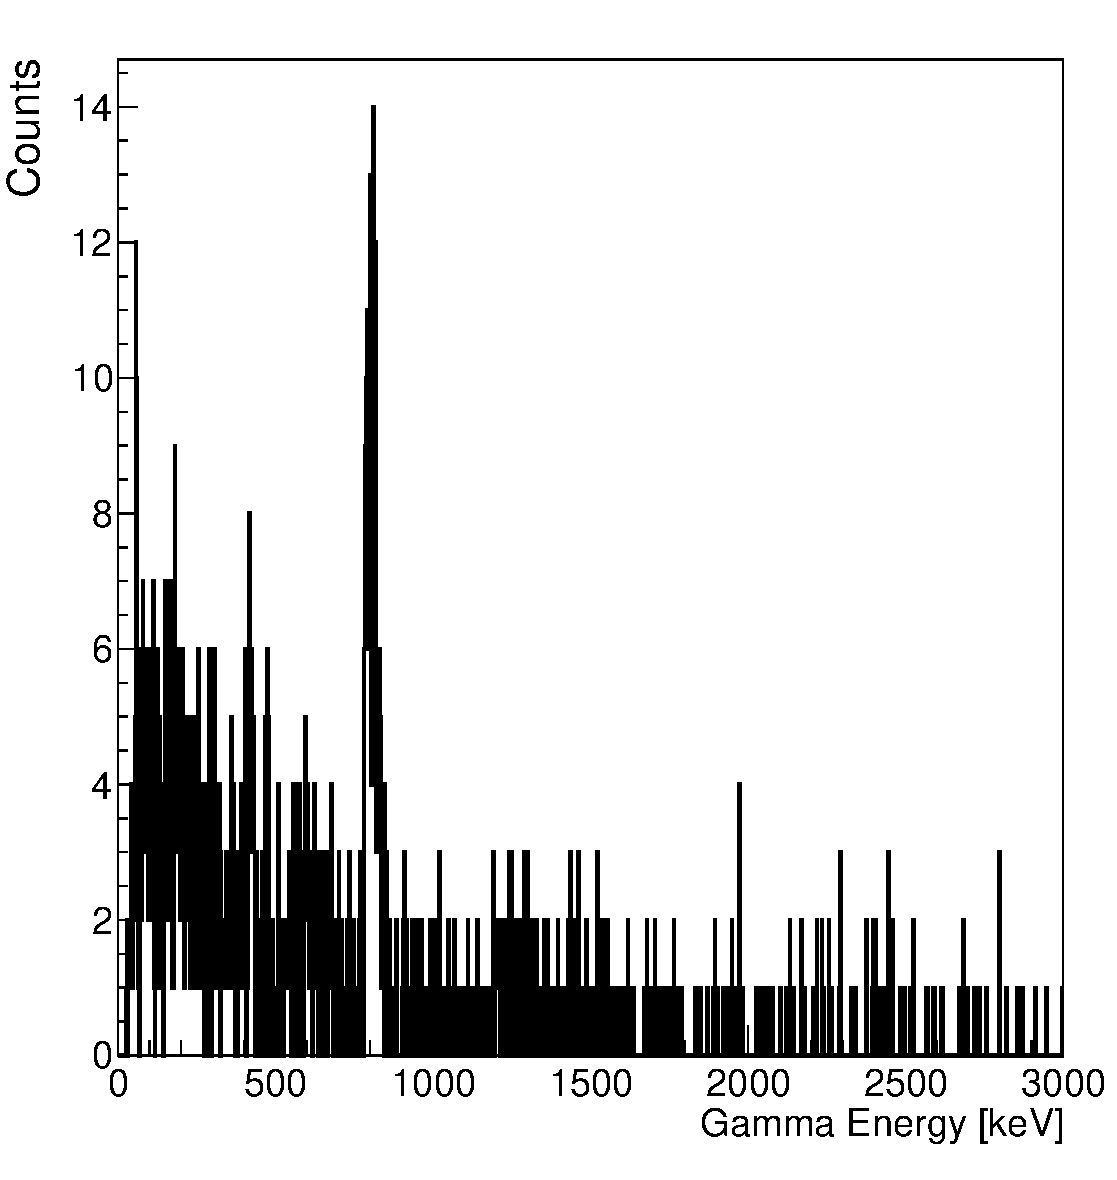
\includegraphics[width=\textwidth]{GammaGated}}
			\end{overlayarea}
		\end{column}
		\begin{column}{0.4\textwidth}
			\begin{overlayarea}{\textwidth}{\textheight}
			\centering
			    \vspace{-0.15\textheight}
			    
				\only<1>{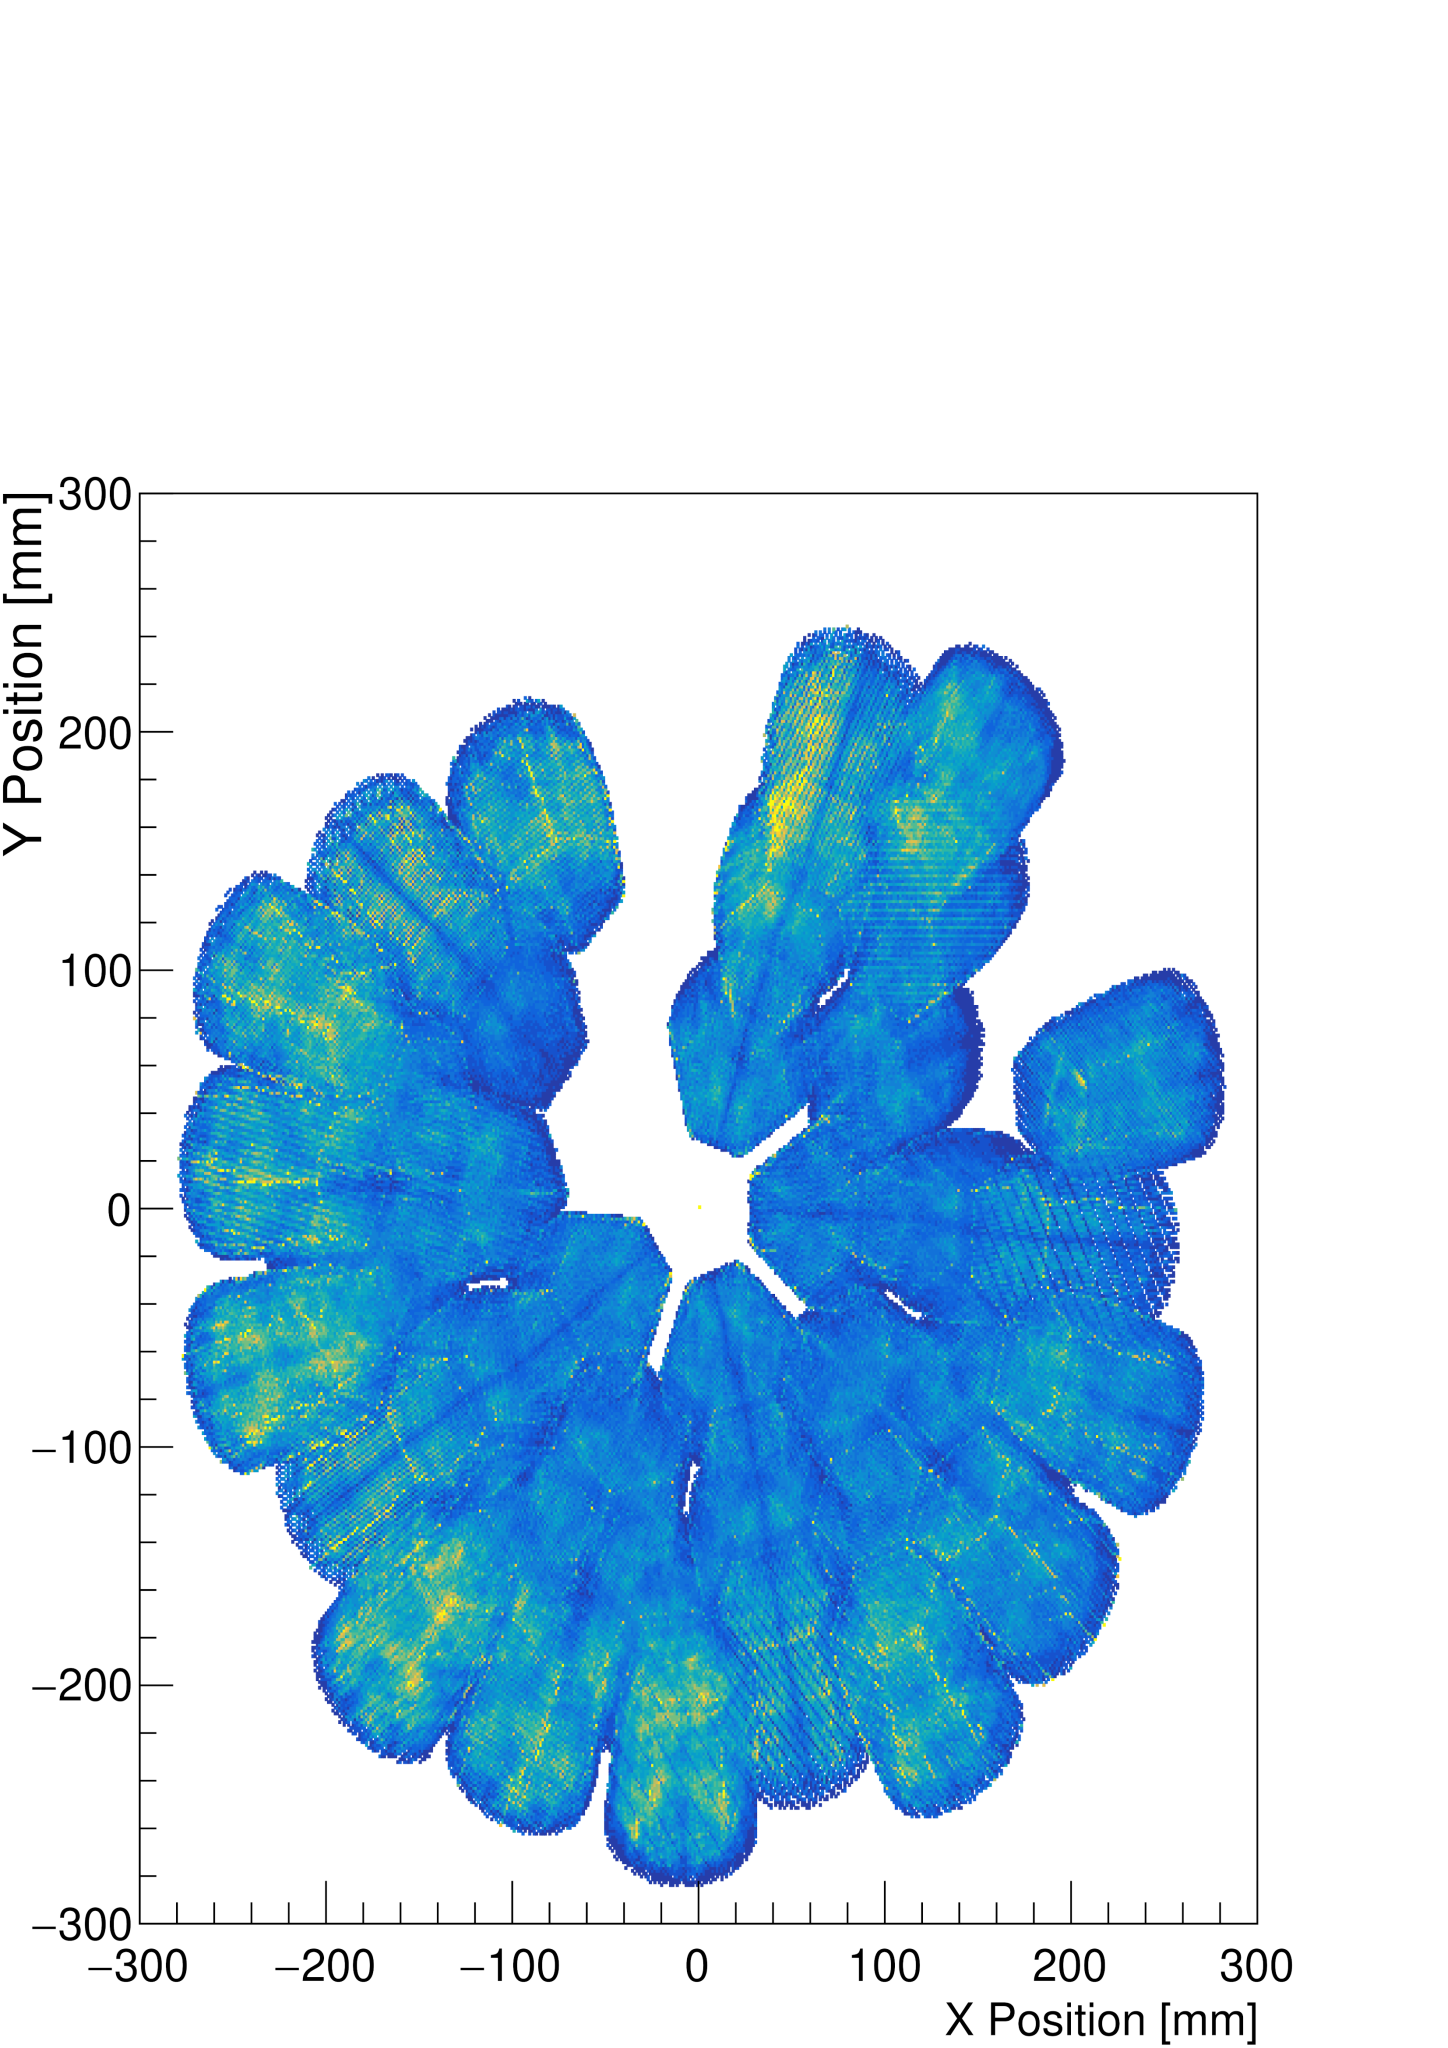
\includegraphics[width=\textwidth]{AGATAimpact.png}
				            Gamma spectrum w/o gate.\\
                            $\mathbf{6.9\ 10^{7}}$~\textbf{ev}.\\	
                            		    
						    }
				\only<2>{   \vspace{0.3\textheight}
							Proton gated spectrum.\\
							$\mathbf{1.6\ 10^{3}}$~\textbf{ev}.\\
							$\downarrow$\\
							\vspace{0.1\textheight}
							\textbf{Doppler Correction Needed.}
							}
		    \end{overlayarea}	
		\end{column}
	\end{columns}
\end{frame}

\begin{frame}{Doppler Correction}
	\vspace{-0.06\textheight}    
    \begin{overlayarea}{\textwidth}{0.1\textheight}
    \centering
    	\only<1>{}   	
	\only<2>{Minimization of resolution with scan over different shifts}   	
	\only<3>{Best Resolution and Energy match with 33 mm shift} 
	\end{overlayarea}
	%\vspace{0.06\textheight}    

   	\begin{columns}
		\begin{column}{0.5\textwidth}
			\begin{overlayarea}{\textwidth}{\textheight}
				\centering
				\only<1-2>{\includegraphics[width=\textwidth]{GammaDP_51shift}}
				\only<3>{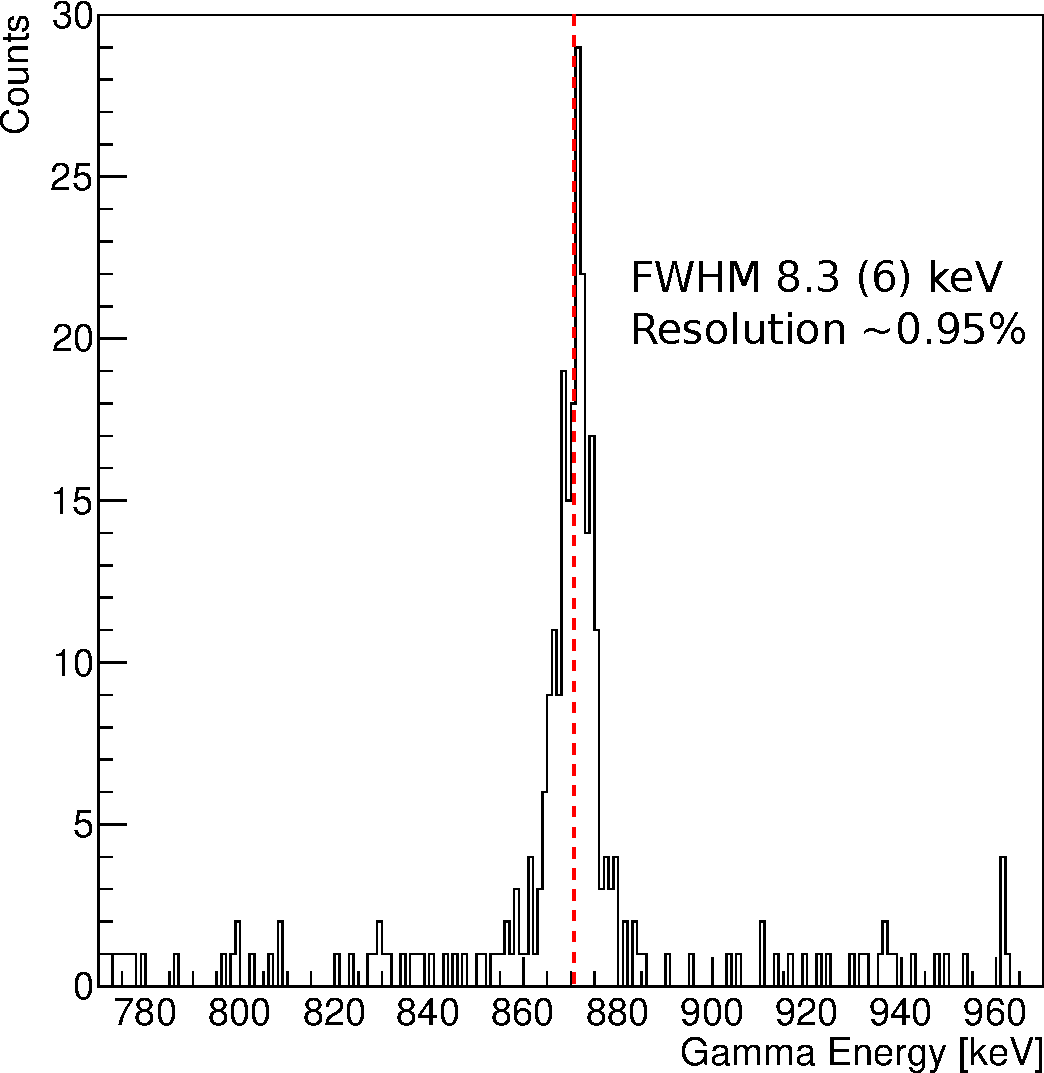
\includegraphics[width=\textwidth]{GammaDP_33shiftResolution}}
			\end{overlayarea}
		\end{column}
		\begin{column}{0.5\textwidth}
			\begin{overlayarea}{\textwidth}{\textheight}
			\centering
			    	\only<1>{
						\vspace{0.15\textheight}			    	        
			    	        \begin{itemize}
							\item Beta computation from proton direction
							\item First interaction from tracking~(51~mm AGATA shift)
						\end{itemize}
						
						The peak is 1.8~keV shifted from\\ 1/2+ state adopted energy.}
				\only<2>{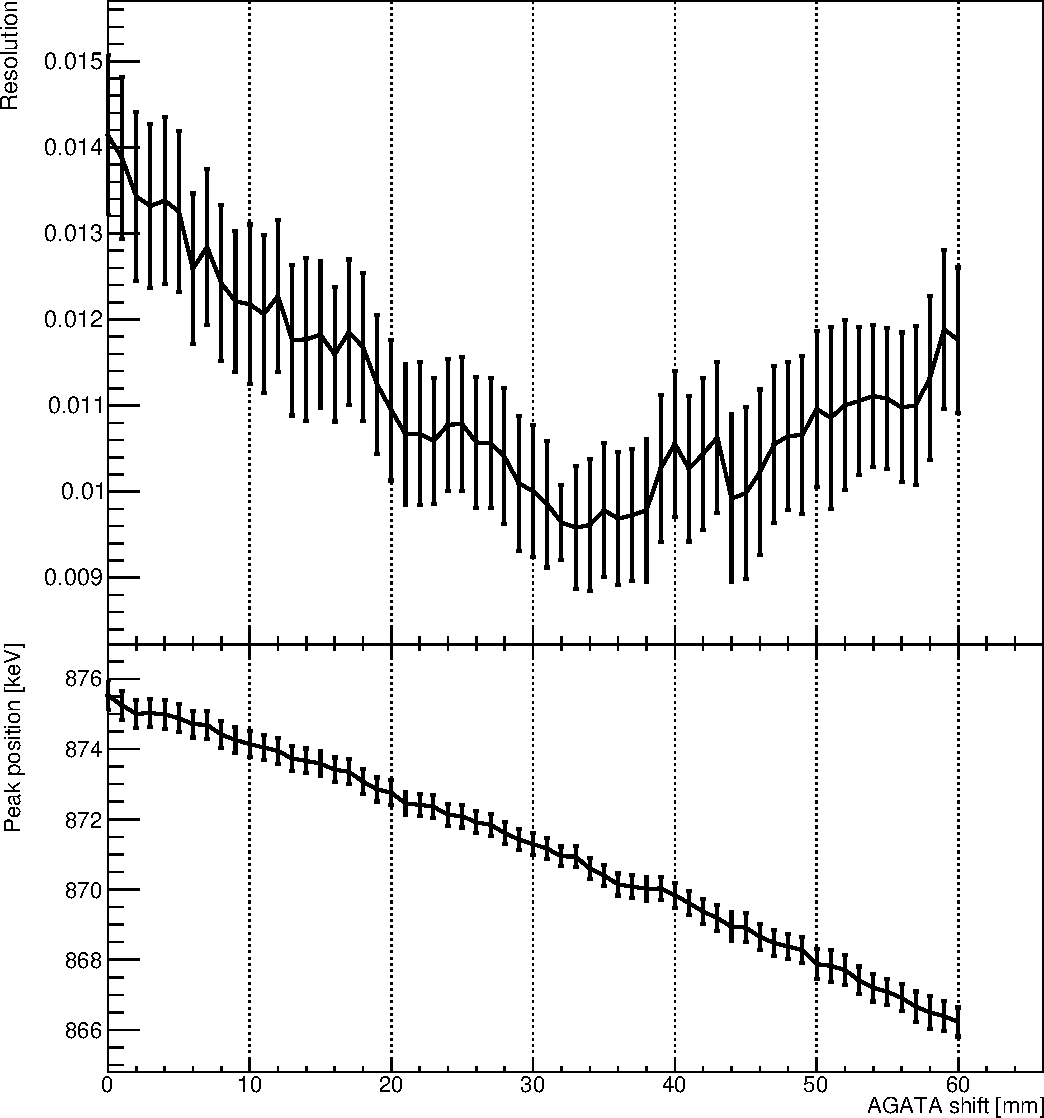
\includegraphics[width=\textwidth]{AGATAShift_ADD_0}}
				\only<3>{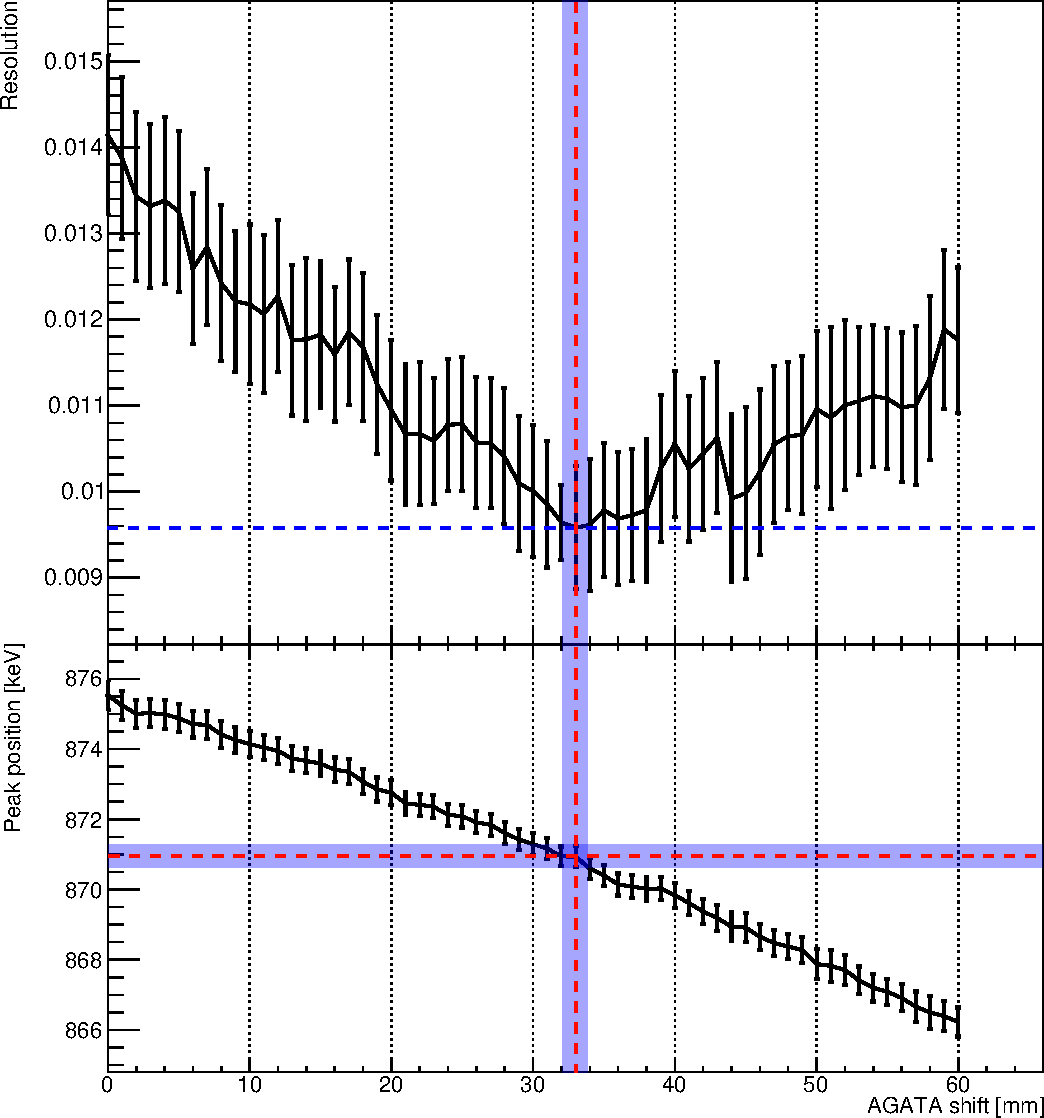
\includegraphics[width=\textwidth]{AGATAShift_ADD_1}}
		    \end{overlayarea}	
		\end{column}
	\end{columns}
\end{frame}

\begin{frame}{Deduced Efficiency}
	\vspace{-0.06\textheight}    
    \centering
	   	
	\vspace{0.06\textheight}    

   	\begin{columns}
		\begin{column}{0.5\textwidth}
			\begin{overlayarea}{\textwidth}{\textheight}
				\centering
				\vspace{0.012\textheight}
				\only<1>{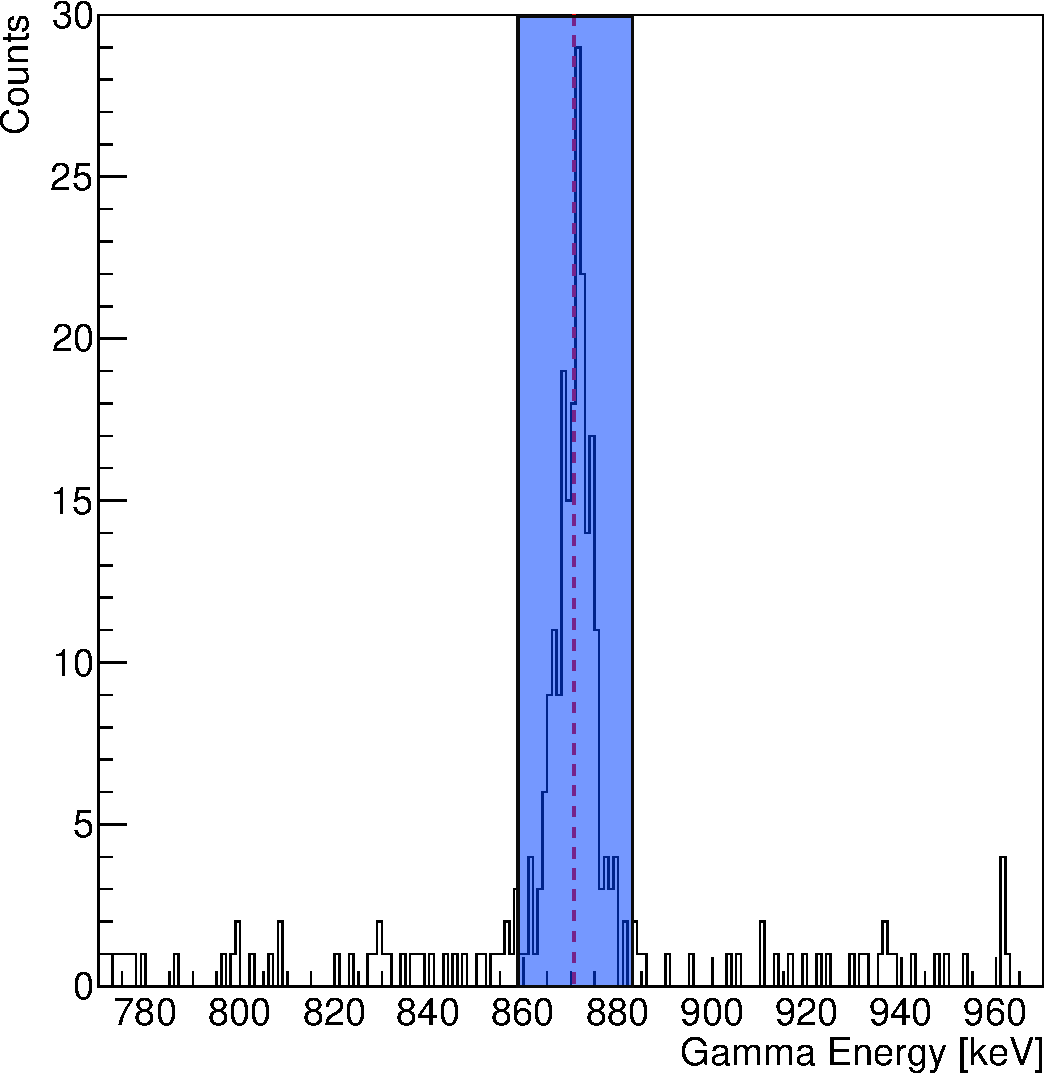
\includegraphics[width=\textwidth]{GammaDP_33shiftInt}}
			\end{overlayarea}
		\end{column}
		\begin{column}{0.5\textwidth}
			\begin{overlayarea}{\textwidth}{\textheight}
			\centering
			    	\vspace{-0.07\textheight}			    	        
			    	        \begin{itemize}
			    	        		\centering
							\item 870~keV excitation peak integral\\ (background removed)\\ $\downarrow$\\ $2562 \pm 50$~protons
							\item{870~keV gamma peak integral (background removed)\\
								  $\downarrow$\\ 
								  \vspace{-0.07\textheight}
								  \begin{align*}
								  \text{\textbf{Add Back}}\ &\rightarrow\ 177\pm 13\ \gamma\\
								  \text{\textbf{Tracking}}\ &\rightarrow\ 160\pm 13\ \gamma
								  \end{align*}
								  }
								\end{itemize}
						\textbf{Efficiency Estimate:}\\
					  \vspace{-0.07\textheight}
						\begin{align*}
								  \text{\textbf{Add Back}}\ &\rightarrow\ 7.0 \pm 0.5\ \%\\
								  \text{\textbf{Tracking}}\ &\rightarrow\ 6.3 \pm 0.5\ \%
						\end{align*}
						
			\end{overlayarea}	
		\end{column}
	\end{columns}
\end{frame}

